%%%%%%%%%%%%%%%%%%%%%%%%%%%%%%%%%%%%%%%%%
% Beamer Presentation
% LaTeX Template
% Version 1.0 (10/11/12)
%
% This template has been downloaded from:
% http://www.LaTeXTemplates.com
%
% License:
% CC BY-NC-SA 3.0 (http://creativecommons.org/licenses/by-nc-sa/3.0/)
%
%%%%%%%%%%%%%%%%%%%%%%%%%%%%%%%%%%%%%%%%%

%----------------------------------------------------------------------------------------
%	PACKAGES AND THEMES
%----------------------------------------------------------------------------------------

\documentclass{beamer}

\mode<presentation> {

% The Beamer class comes with a number of default slide themes
% which change the colors and layouts of slides. Below this is a list
% of all the themes, uncomment each in turn to see what they look like.

%\usetheme{default}
%\usetheme{AnnArbor}
%\usetheme{Antibes}
%\usetheme{Bergen}
%\usetheme{Berkeley}
%\usetheme{Berlin}
%\usetheme{Boadilla}
\usetheme{CambridgeUS}
%\usetheme{Copenhagen}
%\usetheme{Darmstadt}
%\usetheme{Dresden}
%\usetheme{Frankfurt}
%\usetheme{Goettingen}
%\usetheme{Hannover}
%\usetheme{Ilmenau}
%\usetheme{JuanLesPins}
%\usetheme{Luebeck}
%\usetheme{Madrid}
%\usetheme{Malmoe}
%\usetheme{Marburg}
%\usetheme{Montpellier}
%\usetheme{PaloAlto}
%\usetheme{Pittsburgh}
%\usetheme{Rochester}
%\usetheme{Singapore}
%\usetheme{Szeged}
%\usetheme{Warsaw}

% As well as themes, the Beamer class has a number of color themes
% for any slide theme. Uncomment each of these in turn to see how it
% changes the colors of your current slide theme.

%\usecolortheme{albatross}
%\usecolortheme{beaver}
%\usecolortheme{beetle}
%\usecolortheme{crane}
%\usecolortheme{dolphin}
%\usecolortheme{dove}
%\usecolortheme{fly}
%\usecolortheme{lily}
%\usecolortheme{orchid}
%\usecolortheme{rose}
%\usecolortheme{seagull}
%\usecolortheme{seahorse}
%\usecolortheme{whale}
%\usecolortheme{wolverine}


%\setbeamertemplate{footline} % To remove the footer line in all slides uncomment this line
%\setbeamertemplate{footline}[page number] % To replace the footer line in all slides with a simple slide count uncomment this line

%\setbeamertemplate{navigation symbols}{} % To remove the navigation symbols from the bottom of all slides uncomment this line
}
\usepackage[utf8]{inputenc}
\usepackage{amsmath}
\usepackage{graphicx} % Allows including images
\usepackage{booktabs} % Allows the use of \toprule, \midrule and \bottomrule in tables

%----------------------------------------------------------------------------------------
%	TITLE PAGE
%----------------------------------------------------------------------------------------

\title[Planck Stars]{Introduction to Plack Stars} % The short title appears at the bottom of every slide, the full title is only on the title page

\author[Hernández A.]{Alejandro Hernández A. } % Your name
\institute[Uniandes] % Your institution as it will appear on the bottom of every slide, may be shorthand to save space
{
Universidad de los Andes, Bogotá, Colombia \\ % Your institution for the title page
%\medskip
%\textit{a.hernandez105@uniandes.edu.co}\\
%\textit{jd.prada1760@uniandes.edu.co}
 % Your email address
}
\date{November 6, 2015} % Date, can be changed to a custom date

\begin{document}

\begin{frame}
\titlepage % Print the title page as the first slide
\end{frame}

\begin{frame}
\frametitle{Overwiew} % Table of contents slide, comment this block out to remove it
\tableofcontents % Throughout your presentation, if you choose to use \section{} and \subsection{} commands, these will automatically be printed on this slide as an overview of your presentation
\end{frame}

%----------------------------------------------------------------------------------------
%	PRESENTATION SLIDES
%----------------------------------------------------------------------------------------

%------------------------------------------------
\section{Introduction} % Sections can be created in order to organize your presentation into discrete blocks, all sections and subsections are automatically printed in the table of contents as an overview of the talk
%------------------------------------------------

%\subsection{Introduction} % A subsection can be created just before a set of slides with a common theme to further break down your presentation into chunks

\subsection{Black hole solutions}

\section{Regularized Schwarzschild metric}

\subsection{Hayward metric}

\section{Quantum Field Theory}

\subsection{Newtonian Potential}
\subsection{Quantum cosmology remarks}
\subsection{Plank stars}





\begin{frame}
\frametitle{Preliminaries}

\textbf{Einstein Field Equations} \\\

\begin{equation}
\label{field}
R_{\mu \nu} - \frac{1}{2} R g_{\mu \nu} + \Lambda g_{\mu \nu} = 8 \pi T_{\mu \nu}
\end{equation}

\
\\
\
\\

\textbf{Minkowski metric} \\\

\begin{equation}
\label{mink}
ds^2 = -dt^2 + dr^2 + r^2d\Omega ^2
\end{equation}


\end{frame}

%------------------------------------------------

\begin{frame}
\frametitle{Black hole solutions}

\textbf{Classification of Black holes}\\\
\\\


\begin{center}
  \begin{tabular}{| c | c | c |}
    \hline
     & Non-rotating ($J=0$) & Rotating ($J\neq 0$)\\ \hline
    Uncharged ($Q =0 $) & Schwarzschild & Kerr \\ \hline
    Charged ($Q \neq 0$) & Reissner-Nordstr\"om & Kerr-Newman \\
    \hline
  \end{tabular}
\end{center}


\end{frame}

%------------------------------------------------

\begin{frame}[fragile] % Need to use the fragile option when verbatim is used in the slide
\frametitle{Schwarzschild Black hole}

\textbf{Schwarzschild metric}
\begin{equation}
\label{sch}
ds^2 = -\left(1 - \frac{2m}{r} \right) dt^2 + \left(1 - \frac{2m}{r} \right)^{-1}dr^2 + r^2d\Omega ^2
\end{equation}

\
\\
\
\\

\textbf{Kretschmann invariant}
\begin{equation}
\label{kret}
\kappa = R^{\alpha \beta \gamma \delta} R_{\alpha \beta \gamma \delta} = \frac{48m^2}{r^6}
\end{equation}

\end{frame}

%------------------------------------------------

\begin{frame}
\frametitle{Regularized Schwarzschild metric}
According to \cite{hayward}, we cand find metrics that are:

\begin{itemize}
\item Spherically symmetric.
\item Static.
\item Asymptotically flat (minkowski).
\item \textbf{Have regular center.}
\end{itemize}

The resulting stress-energy tensor is physically reasonable, satisfies the weak energy condition and has components that are bounded and fall off appropriately at large distance.

%OJO Condiciones de energía, y el comentario de horizontes de Cauchy.


\end{frame}

%------------------------------------------------



%------------------------------------------------

\begin{frame}
\frametitle{Regularized Schwarchild metric}
Consider a static, spherically symmetric metric of the form:

\begin{equation}
ds^2 = -F(r)dt^2 + \frac{1}{F(r)}dr^2 + r^2d\Omega ^2
\end{equation}

We demand

\begin{equation}
F(r) \sim 1 - \frac{2m}{r}\ \ \ as\ \ \ r \rightarrow \infty
\end{equation}

\begin{equation}
F(r) \sim 1 - \frac{r^2}{l^2}\ \ \ as\ \ \ r \rightarrow 0
\end{equation}

%OJO - l densidad de energía y hubble length.

\end{frame}

%------------------------------------------------

\begin{frame}
\frametitle{Hayward metric}
The so called Hayward metric \cite{hayward} satisfies all the required properties and is given by:

\begin{equation}
\label{hayw}
F(r) = 1 - \frac{2mr^2}{r^3 + 2ml^2}
\end{equation}

For this metric, the Kretschmann invariant is

\begin{equation}
OJO
\end{equation}



%where $l$ encodes the central energy density $\frac{3}{8\pi l^2}$

%Analyzing the zeros of $g_{tt} = F(r)$


\end{frame}


\begin{frame}
\frametitle{Hayward metric}

Analyzing the zeros of $F(r)$, we get a critical mass $m_{*} = \frac{3\sqrt{3}}{4}l$ and a radius $r_{*} = \sqrt{3}l$.

%\begin{itemize}
%\item No zeros if $m < m_{*}$. %($\leftrightsquigarrow$ Regular space time with the same causal structure as a flat space-time).
%\item One double zero at $r = r_{*}$ if $m = m_{*}$.
%%($\leftrightsquigarrow$ Regular extreme black hole with degenerate Killing horizon).
%\item Two simple zeros at $r = r_{\pm}$ if $m > m_{*}$.
%%($\leftrightsquigarrow$ Regular nonextreme black hole with both outer and inner Killing horizons located at $r_{+} \approx 2m$ and $r_{-} \approx l$ for $m \gg m_{*}$). OJO con el mass gap.
%\end{itemize}

\begin{figure}[h!]
	\centering
	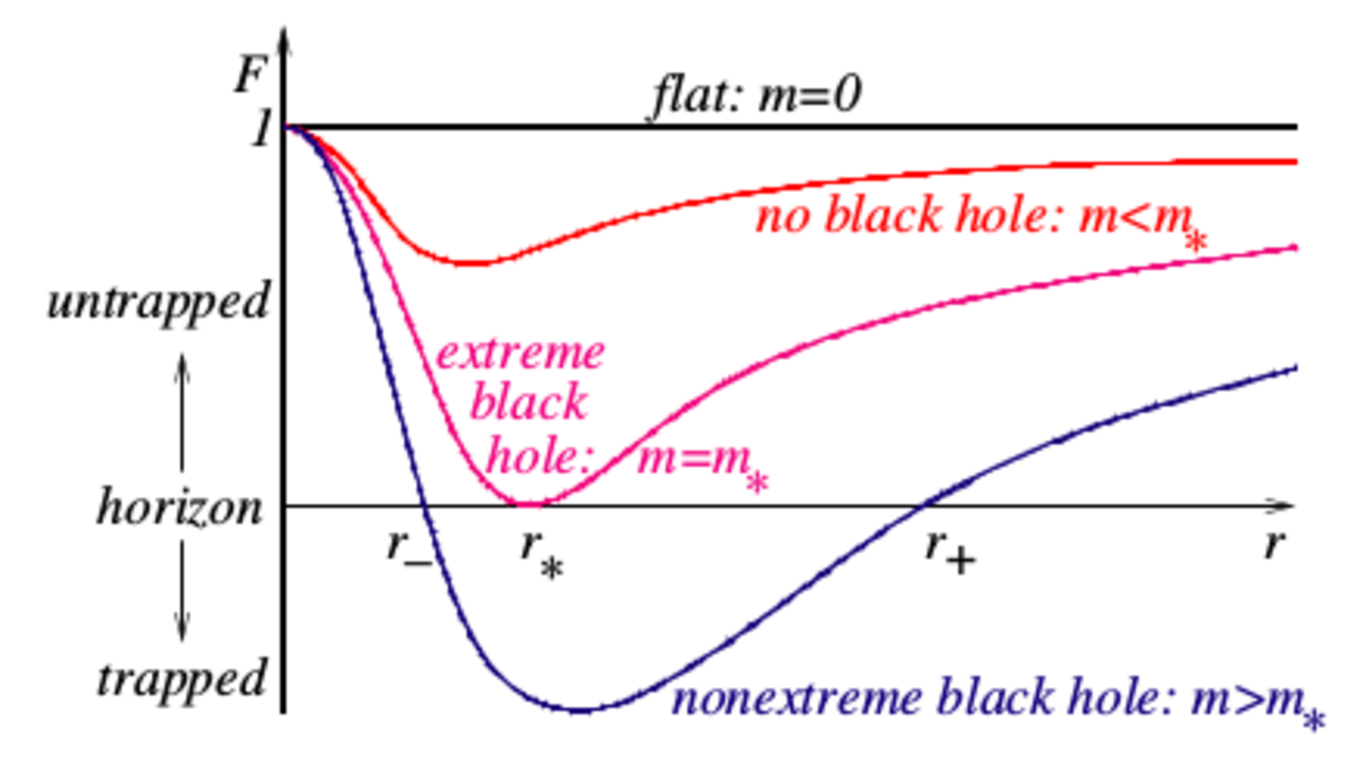
\includegraphics[width=0.7\textwidth]{F(r)}
	\caption{Behavior\footnote{Image taken from \cite{hayward}.} of $g_{tt} = F(r)$ for different values of the parameter $m$.}
	
\end{figure}

\end{frame}

%\begin{frame}
%\frametitle{Hayward metric}
%If we use field equations \ref{field}, we note that this metric is supported by density $-T^{t}_{t}$, radial pressure $T^{r}_{r}$, and transverse pressure $T^{\theta}_{\theta} = T^{\phi}_{\phi}$ given by:
%
%\begin{equation}
%G^{t}_{t} = G^{r}_{r} = - \frac{12l^2m^2}{\left( r^3 + 2l^2m \right)^2}
%\end{equation}
%
%\begin{equation}
%G^{\theta}_{\theta} = G^{\phi}_{\phi} = \frac{24\left( r^3 - l^2m \right)l^2m^2}{\left( r^3 + 2l^2m \right)^3}
%\end{equation}
%
%%OJO They fall off very rapidly $\mathcal{O}(r^{-6})$
%
%%OJO Con la radiación
%
%\end{frame}

\begin{frame}
\frametitle{Quantum Field Theory}
Spacetime metric describing 'non-singular' black holes are commonly studied in the literature \cite{effective,planck stars} as effective modification to the Schwarzschild solution that mimic quantum gravity effects removing the central singuarity.\\\

To begin with, two insights from quantum cosmology \cite{ashtekar}:

%OJO Especificar que al hablar de gravedad cuántica es realmente teoría cuántica de campos efectiva.
\begin{itemize}
\item The onset of quantum gravitational effects is when energy density reaches the Plank scale ($\sim 5.155 \cdot 10^{96}\ \frac{kg}{m^3}$).\\\

\item The dominant quantum effect at high density is a strong pressure, sufficient to counterbalance weight and reverse gravitational collapse.
\end{itemize} 
\end{frame}

%\begin{frame}
%\frametitle{Plack scale}
%
%Planck scale is given by\\\	
%\begin{center}
%  \begin{tabular}{| c | c |}
%    \hline
%    \textbf{Quantity} & \textbf{SI equivalent} \\ \hline
%    Planck time & $t_{p} = 5.39121 \cdot 10^{-44} s$\\ \hline
%    Planck mass & $m_{p} = 2.17645 \cdot 10^{-8} kg$\\ \hline
%    Planck length & $l_{p} = 1.616252 \cdot 10^{-35} m$\\ \hline
%  \end{tabular}
%\end{center}
%\
%\\
%\
%\\
%
%and the Plack density is the quotient
%
%\begin{equation}
%\rho _{p} = \frac{m_{p}}{l_{p}^3} \approx 5.155 \cdot 10^{96}\ \frac{kg}{m^3}
%\end{equation}
%\end{frame}

\begin{frame}
\frametitle{Quantum Field theory}

For a black hole, the previous arguments imply that matter's collapse can be stopped before the central singularity is formed, yielding the formation of a central core, called a \textbf{Planck star}.

%OJO En otras palabras, podemos definir una estrella de Plack
\end{frame}
%------------------------------------------------

\begin{frame}
\frametitle{References}
\footnotesize{
\begin{thebibliography}{99} % Beamer does not support BibTeX so references must be inserted manually as below

\bibitem{hayward} Hayward, S.A.: Formation and Evaporation of regular black holes. Phys. Rev. Lett. \textbf{96}, 31103 (2006).

\bibitem{effective} De Lorenzo, T., Pacilio, C., Rovelli, C., Speziale, S.: On the effective metric of a Planck star. Gen. Relativ. Gravit. \textbf{47}, 41 (2015).

\bibitem{planck stars} Rovelli, C., Vidotto, F.: Planck Stars. Int. J. Mod. Phys. D. \textbf{23}, 1142026, (2014).

\bibitem{ashtekar} Ashtekar, A., Pawlowski, T., Singh, P., Vandersloot, K.: Loop quantum cosmology of k=1 FRW models. Phys. Rev. D \textbf{75},24035 (2007).

\bibitem{mazur} Mazur, P. O., Mottola, E.: Gravitational condensate stars: An alternative to black holes, 

\end{thebibliography}
}
\end{frame}

%------------------------------------------------

\begin{frame}
\Huge{\centerline{The End}}
\end{frame}

%----------------------------------------------------------------------------------------

\end{document} 